\section{Results}\label{Results}
\subsection{Datasets}
\begin{table}[htbp]
\centering
\caption{The details of the dataset information.}
\label{tab: Results, Datasets}
\begin{tabular*}{\tblwidth}{CCCC}
\toprule
\multicolumn{4}{c}{\textbf{HF datasets}} \\
Group & Age($\bar x \pm sd$) & Sex & Length(min)\\ 
\midrule
Healthy&$24$&Male&27.0\\
Healthy&$26\pm 2$&Female&54.0\\
HF&$72.6\pm12.0$&Male&34.8\\
HF&$77.9\pm 11.1$&Female&36.8\\
\midrule
\end{tabular*}
% \begin{tabular*}{\tblwidth}{CC|CC}
% \multicolumn{2}{l|}{Multi-region fusion auscultation}&\multicolumn{2}{l}{Mitral valve auscultation} \\
% \midrule
% Healthy&540&Healthy&1620\\
% HF&389&HF&1379\\
% \midrule
% \end{tabular*}
\begin{tabular*}{\tblwidth}{LL}
\multicolumn{2}{c}{\textbf{Denoising dataset}} \\
Description & Length(s) \\ 
\midrule
Systolic murmur& $68$ \\ 
Functional aortic stenosis& $4$ \\ 
Musical noise& $23$ \\ 
Organic mitral regurgitation& $59$ \\ 
Functional mitral stenosis& $9$ \\ 
Organic mitral stenosis& $9$ \\ 
Diplogue& $39$ \\ 
Paradoxically divided& $13$ \\ 
Varied S1 & $23$ \\ 
Weak S1 & $3$\\
Split S1& $4$ \\
Strong S1& $6$\\
Weak S2 & $29$\\
Split S2 & $12$ \\ 
Ventricular septal defect& $9$ \\ 
Open flap sound& $10$ \\ 
Late contraction& $9$ \\ 
Relative mitral regurgitation& $4$ \\
Sinus bradycardia& $7$\\
Sinus tachycardia& $4$ \\
Functional pulmonary regurgitation & $3$\\
Pulmonary stenosis & $67$\\
Diastolic tetratone & $15$\\
Continuous murmur & $15$\\
Overlapping galloping sound & $9$\\
Pendulum sound& $6$\\
\midrule
\end{tabular*}
\begin{tabular*}{\tblwidth}{LL}
\multicolumn{2}{c}{\textbf{Yaseen dataset}} \\
Description & Number \\ 
\midrule
Aortic Stenosis& 200 \\ 
Mitral Regurgitation& 200 \\ 
Mitral Stenosis& 200 \\ 
Mitral Valve Prolapse& 200 \\ 
Normal& 200 \\ 
\bottomrule
\end{tabular*}
\end{table}
Tab. \ref{tab: Results, Datasets} shows the details of the dataset in this paper. The details include the age and gender composition of auscultation volunteers, and case descriptions for the denoising dataset. Auscultation dataset contains 2999  recordings from heart failure patients, each with rich annotations, and are publicly accessible on \href{https://github.com/jimmytju/AHF-Rapid-Diagnosis/Database}{https://github.com/jimmytju/AHF-Rapid-Diagnosis/Database}.
\subsection{Preprocessing}
Firstly, we conduct an analysis to determine the average SNR under various combinations of wavelet bases and decomposition layers, using a coefficient shrinkage function based on the 20\% modulo maximum hard threshold. The results of this analysis are presented in Fig. \ref{FIG:wavelet}, which clearly indicates that the Sym8 base at the 7-layer decomposition level yields the most effective denoising results among the tested methods.

Secondly, we further investigate the average SNR across different shrinkage functions and threshold values while maintaining the sym8 base at the 7-layer decomposition level. Our findings indicate that the use of the 20\% modulo maximum with the $f_{self}$ threshold function emerged as the optimal denoising method.

Finally, the average SNR of the denoising algorithm proposed in this paper is 7.8 dB.
\begin{figure}
	\centering
	\begin{subfigure}{1\linewidth}
		\centering
		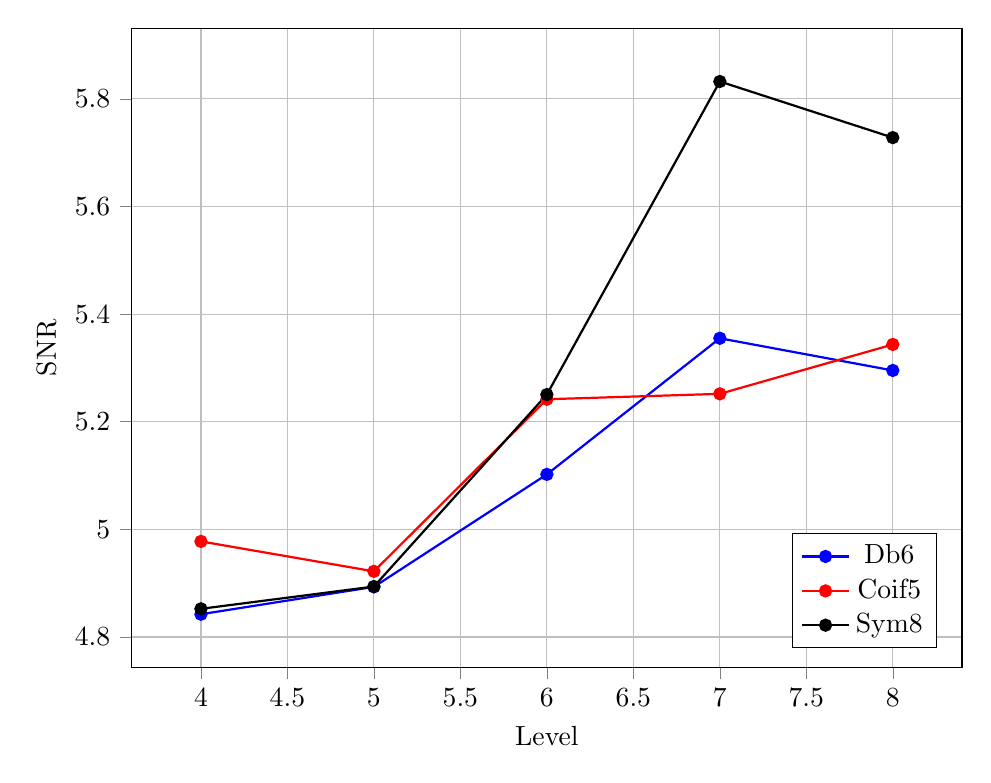
\begin{tikzpicture}
\begin{axis}[
    tick align=outside,
    xtick pos=bottom,ytick pos=left,
    height=0.8\textwidth,
    width=1\textwidth,    
    grid=major,
    % title={Choice of base and levels},
    xlabel={Level},
    ylabel={SNR},
    legend pos=south east,
            ymajorgrids=true,]
\addplot[
    color=blue,
    mark=*,thick, 
    ]
    coordinates {
	(4,4.842219216)
	(5,4.893083055)
	(6,5.102156965)
	(7,5.355110876)
	(8,5.295298758)
    };
\addplot[
    color=red,
    mark=*,thick, 
    ]
    coordinates {    
	(4,4.977584716)
	(5,4.921934414)
	(6,5.241793852)
	(7,5.251832822)
	(8,5.34360019)
    };
\addplot[
    color=black,
    mark=*,thick
    ]
    coordinates {
	(4,4.852302411)
	(5,4.893708271)
	(6,5.250521718)
	(7,5.832332806)
	(8,5.728034433)
    };
\legend{Db6,Coif5,Sym8}
\end{axis}
\end{tikzpicture}
		\caption{Choice of base and levels}
		\label{FIG:wavelet.a}%文中引用该图片代号
	\end{subfigure}\\
	\quad
	\centering
	\begin{subfigure}{1\linewidth}
		\centering
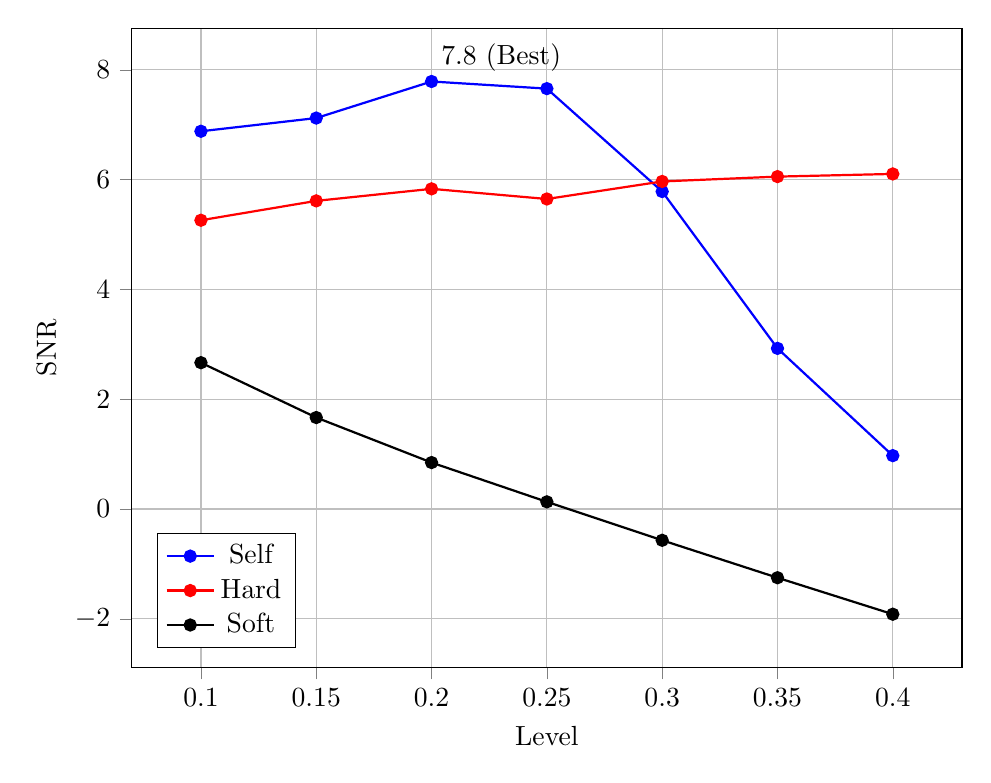
\begin{tikzpicture}
\begin{axis}[
    tick align=outside,
    xtick pos=bottom,ytick pos=left,
    height=0.8\textwidth,
    width=1\textwidth,
    % title={Choice of threshold parameters},
    xlabel={Level},
    ylabel={SNR},
    legend pos=south west,    
    grid=major,
    ymajorgrids=true,]
\addplot[
    color=blue,
    mark=*,thick,
    ]
    coordinates {
(0.1,6.881196846)
(0.15,7.121921467)
(0.2,7.788052276)
(0.25,7.658138472)
(0.3,5.783732988)
(0.35,2.926190942)
(0.4,0.971827728)
    };
\addplot[
    color=red,
    mark=*,thick,
    ]
    coordinates { 
(0.1,5.260228914)
(0.15,5.613376992)
(0.2,5.832332806)
(0.25,5.647585743)
(0.3,5.967033361)
(0.35,6.055329555)
(0.4,6.104046502)
    };
\addplot[
    color=black,
    mark=*,thick,
    ]
    coordinates {
(0.1,2.66541873)
(0.15,1.666208437)
(0.2,0.845928378)
(0.25,0.130262098)
(0.3,-0.570100528)
(0.35,-1.252319888)
(0.4,-1.91680774)
    };
\legend{Self,Hard,Soft}
% Annotation for the point (0.2, 7.718052276)
\node[above right] at (axis cs:0.2,7.788052276) {7.8 (Best)};
\end{axis}
\end{tikzpicture}
		\caption{Choice of threshold parameters}
		\label{FIG:wavelet.b}%文中引用该图片代号
	\end{subfigure}
\caption{\textbf{Wavelet denoising of short signal.} (\textbf{a}) Best: wavelet denoising with sym8 base at 7-layer decomposition. (\textbf{b}) Best: wavelet denoising with 20\% modulo maximum $f_{self}$.}
\label{FIG:wavelet}
\end{figure}
\subsection{Multi-region fusion auscultation}
The quality of models refers to Eq.\ref{eq:Acc}: Accuracy (Acc), Eq.\ref{eq:Se}: Sensitivity (Se),  Eq.\ref{eq:Sp}: Specificity (Sp) and Eq.\ref{eq:F1}: F1-Score.
\begin{equation}
\begin{split}
    Acc= \frac{TP+TN}{TP+FP+TN+FN}
\end{split}
\label{eq:Acc}
\end{equation}
\begin{equation}
\begin{split}
	Se=   \frac{TP}{TP+FN}
\end{split}
\label{eq:Se}
\end{equation}
\begin{equation}
\begin{split}
  Sp=  \frac{TN}{TN+FP}
\end{split}
\label{eq:Sp}
\end{equation}
\begin{equation}
\begin{split}
  F1-Score= 2\times\frac{Se\times Sp}{Se+Sp} 
\end{split}
\label{eq:F1}
\end{equation}\par

Tab.\ref{tab:HF Diagnosis 10-fold Results} presents the classification results on the HF-Diagnosis dataset and the public Yassen dataset, comparing the performance of three models: DenseHF-Net, ResNet-18, and MobileNetV1-28. 

\begin{table*}
    \centering
    \caption{Classification results of HF-Diagnosis dataset and public Yassen Dataset.}
    \label{tab:HF Diagnosis 10-fold Results}
    \begin{tabular*}{\tblwidth}{LCCLCCLCC}
    \toprule
    \multicolumn{9}{c}{\textbf{Multi-region fusion auscultation results}} \\
    \textbf{DenseHF-Net(ours)}&\multicolumn{2}{c|}{$Average\pm sd$}&ResNet-18&\multicolumn{2}{c|}{$Average\pm sd$}&MobileNetV1-28&\multicolumn{2}{c}{$Average\pm sd$}\\
    \hline
    $Acc(\%)$&\multicolumn{2}{c|}{$99.25\pm0.71$}&$Acc(\%)$&\multicolumn{2}{c|}{$98.71\pm1.26$}&$Acc(\%)$&\multicolumn{2}{c}{$99.14\pm0.65$}\\
    $Se(\%)$&\multicolumn{2}{c|}{$98.97\pm1.22$}&$Se(\%)$&\multicolumn{2}{c|}{$99.09\pm0.92$}&$Se(\%)$&\multicolumn{2}{c}{$100.00\pm0.00$}\\
    $Sp(\%)$&\multicolumn{2}{c|}{$99.44\pm0.75$}&$Sp(\%)$&\multicolumn{2}{c|}{$98.10\pm2.68$}&$Sp(\%)$&\multicolumn{2}{c}{$97.95\pm1.54$}\\
    $F1-Score(\%)$&\multicolumn{2}{c|}{$99.10\pm0.64$}&$F1-Score(\%)$&\multicolumn{2}{c|}{$98.59\pm1.49$}&$F1-Score(\%)$&\multicolumn{2}{c}{$98.97\pm0.78$}\\
    \end{tabular*}
    \begin{tabular*}{\tblwidth}{LCCLCCLCC}
            \multicolumn{9}{c}{\textbf{Mitral valve auscultation results}} \\
    \textbf{DenseHF-Net(ours)}&\multicolumn{2}{c|}{$Average\pm sd$}&ResNet-18&\multicolumn{2}{c|}{$Average\pm sd$}&MobileNetV1-28&\multicolumn{2}{c}{$Average\pm sd$}\\
    \hline
    $Acc(\%)$&\multicolumn{2}{c|}{$92.60\pm1.11$}&$Acc(\%)$&\multicolumn{2}{c|}{$91.33\pm2.48$}&$Acc(\%)$&\multicolumn{2}{c}{$90.73\pm1.80$}\\
    $Se(\%)$&\multicolumn{2}{c|}{$92.68\pm0.88$}&$Se(\%)$&\multicolumn{2}{c|}{$92.32\pm2.59$}&$Se(\%)$&\multicolumn{2}{c}{$90.68\pm2.49$}\\
    $Sp(\%)$&\multicolumn{2}{c|}{$92.53\pm2.08$}&$Sp(\%)$&\multicolumn{2}{c|}{$90.20\pm4.49$}&$Sp(\%)$&\multicolumn{2}{c}{$90.80\pm2.97$}\\
    $F1-Score(\%)$&\multicolumn{2}{c|}{$92.01\pm2.15$}&$F1-Score(\%)$&\multicolumn{2}{c|}{$91.17\pm2.58$}&$F1-Score(\%)$&\multicolumn{2}{c}{$90.69\pm1.75$}\\
    \end{tabular*}
    \begin{tabular*}{\tblwidth}{l|CCCCCCCCCCCC}
            \multicolumn{13}{c}{\textbf{Yaseen dataset results}} \\
            \multicolumn{1}{c}{}&\multicolumn{4}{c}{\textbf{DenseHF-Net(ours)}}&\multicolumn{4}{c}{ResNet-18}& \multicolumn{4}{c}{MobileNetV1-28} \\
            \cmidrule{2-5}\cmidrule{6-9}\cmidrule{10-13}
            \multicolumn{1}{c}{}&AS&MR&MS&MVP&AS&MR&MS&MVP&AS&MR&MS&MVP\\
            \hline
            $Acc(\%)$&91.25&58.75&75.00&63.75&92.50&88.75&95.00&83.75&82.50&92.50&85.00&88.75\\
            $Se(\%)$&	90.00&		97.50&	75.00&	97.50&95.00&	80.00&	90.00&		80.00&	87.50&	87.50&			87.50&	87.50\\
            $Sp(\%)$&	92.50&		20.00&	75.00&	30.00&90.00&	97.50&	100.00&		87.50&	77.50&	97.50&			82.50&	90.00\\
            $F1-Score(\%)$&	91.23&		33.19&	75.00&	45.88&92.43&	87.89&	94.74&		83.58&	82.20&	92.23&			84.93&	88.73\\
            \bottomrule
    \end{tabular*}
    \end{table*}
DenseHF-Net achieves the highest accuracy (99.25\% ± 0.71\%) and specificity (99.44\% ± 0.75\%), demonstrating strong classification performance with an F1-score of 99.10\% ± 0.64\%. In comparison, ResNet-18 has an accuracy of 98.71\% ± 1.26\% with lower specificity (98.10\% ± 2.68\%), though its sensitivity is close to DenseHF-Net. MobileNetV1-28 excels in sensitivity (100.00\% ± 0.00\%) but has slightly lower specificity (97.95\% ± 1.54\%), with overall performance similar to DenseHF-Net. In summary, DenseHF-Net offers the best balance between sensitivity and specificity, making it the preferred model for HF-Diagnosis tasks.

Fig.\ref{FIG:Average curve} provides a comprehensive overview of the average performance across the mitral valve auscultation dataset. Notably, ResNet-18 and MobileNetV1-28 exhibit comparable performance, while DenseHF-Net exhibits the most rapid rate of improvement. Importantly, all three models exhibit effective convergence of the loss function. It is worth highlighting that both ResNet-18 and MobileNetV1-28 demonstrate similar performance trends, with DenseHF-Net demonstrating the fastest convergence among them.

\begin{figure*}[h]
	\centering
	\begin{subfigure}{0.48\linewidth}
		\centering
		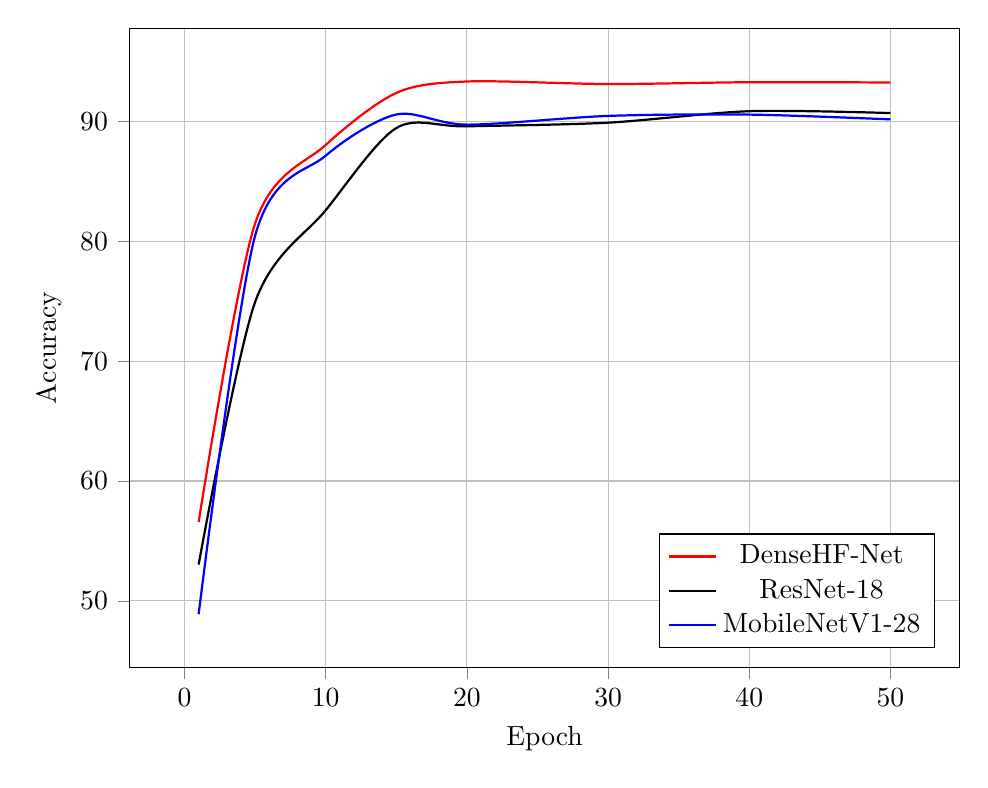
\begin{tikzpicture}
\begin{axis}[
    tick align=outside,
    xtick pos=bottom,ytick pos=left,
    height=0.8\textwidth,
    width=1\textwidth,
    % title={Acc},
    grid=major,
    xlabel={Epoch},
    ylabel={Accuracy},
    xtick={0,10,20,30,40,50},
    ytick={40,50,60,70,80,90,100},
    legend pos=south east,
    ymajorgrids=true,
    % ymajorgrids=true,
    % grid style=dashed,
]
\addplot[
    color=red,
    thick,smooth
    ]
    coordinates {
    (1,56.57439232)
    (5,81.50844994)
    (10,88.05410233)
    (15, 92.39710159301757)
    (20,93.35144958)
    (30,93.14015732)
    (40,93.29104004)
    (50,93.26886444)
    };
\addplot[
    color=black,thick,smooth 
    ]
    coordinates {
    (1,53.03143158)
    (5,74.94425697)
    (10,82.60405884)
    (15, 89.46658782958984)
    (20,89.60950089)
    (30,89.91489792)
    (40,90.87188721)
    (50,90.71563797)
    };
    

\addplot[
    color=blue,
    thick,smooth
    ]
    coordinates {    
    (1,48.88370552)
    (5,80.47420158)
    (10,87.15834885)
    (15, 90.59580764770509)
    (20,89.75154495)
    (30,90.47862091)
    (40,90.58779678)
    (50,90.18920288)
    };

\legend{DenseHF-Net,ResNet-18,MobileNetV1-28}
    
\end{axis}
\end{tikzpicture}
		\caption{Mitral valve auscultation testing accuracy.}
		\label{FIG:Average curve.a}%文中引用该图片代号
	\end{subfigure}
	\begin{subfigure}{0.48\linewidth}
		\centering
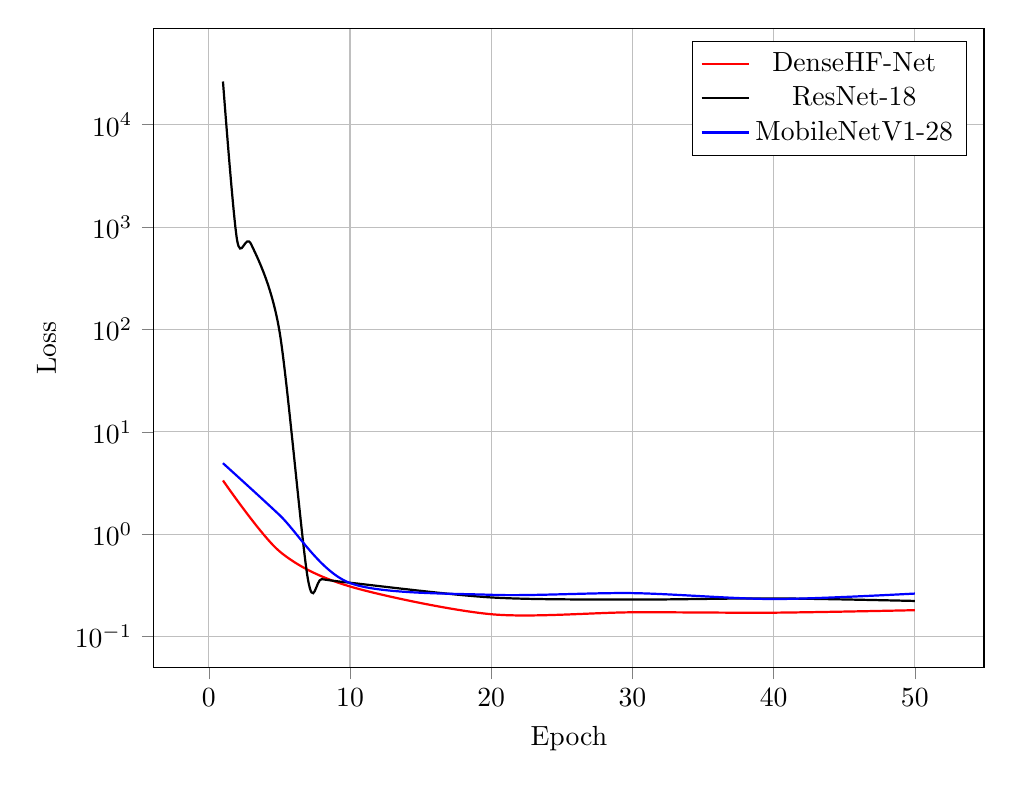
\begin{tikzpicture}
    \begin{axis}[
        tick align=outside,
        xtick pos=bottom,ytick pos=left,
    height=0.8\textwidth,
    width=1\textwidth,
        % title={Acc},
        xlabel=Epoch,
        xtick={0,10,20,30,40,50},
        ytick={0.1,1,10,100,1000,10000},
        ylabel=Loss,
        ymode=log,grid=major,
        log basis y={10},
        ymajorgrids=true,
    % % grid style=dashed,
]
\addplot[
    color=red,thick,smooth
    ]
    coordinates {
    (1,3.355206448)
    (5,0.682259059)
    (10,0.309049669)
    (20,0.165604091)
    (30,0.172943516)
    (40,0.171498471)
    (50,0.18135123)
    };
\addplot[
    color=black,thick,smooth
    ]
    coordinates {
    (1,26451.85823)
    (2,747.1451227188109)
    (3,678.9670787334442)
    (5,96.63756926)
    (7, 0.3756330966949463)
    (8, 0.36473832577466964)
    (10,0.336178899)
    (20,0.241552852)
    (30,0.23027658)
    (40,0.236524488)
    (50,0.223223896)
    };
\addplot[
    color=blue,thick, smooth
    ]
    coordinates {    
    (1,4.946103889)
    (5,1.543885893)
    (10,0.33396288)
    (20,0.25623516)
    (30,0.266215268)
    (40,0.233064194)
    (50,0.263508695)
    };

\legend{DenseHF-Net,ResNet-18,MobileNetV1-28}
    \end{axis}
\end{tikzpicture}
		\caption{Mitral valve auscultation testing loss value.}
		\label{FIG:Average curve.b}%文中引用该图片代号
	\end{subfigure}
\caption{\textbf{Average 10-fold CV history.} (\textbf{a}) Average testing accuracy of three models. (\textbf{b}) Average testing loss of three models (without augmentation).}
\label{FIG:Average curve}
\end{figure*}

\begin{figure*}[htbp]
    \centering
    \begin{subfigure}[b]{0.45\textwidth}
        \centering
        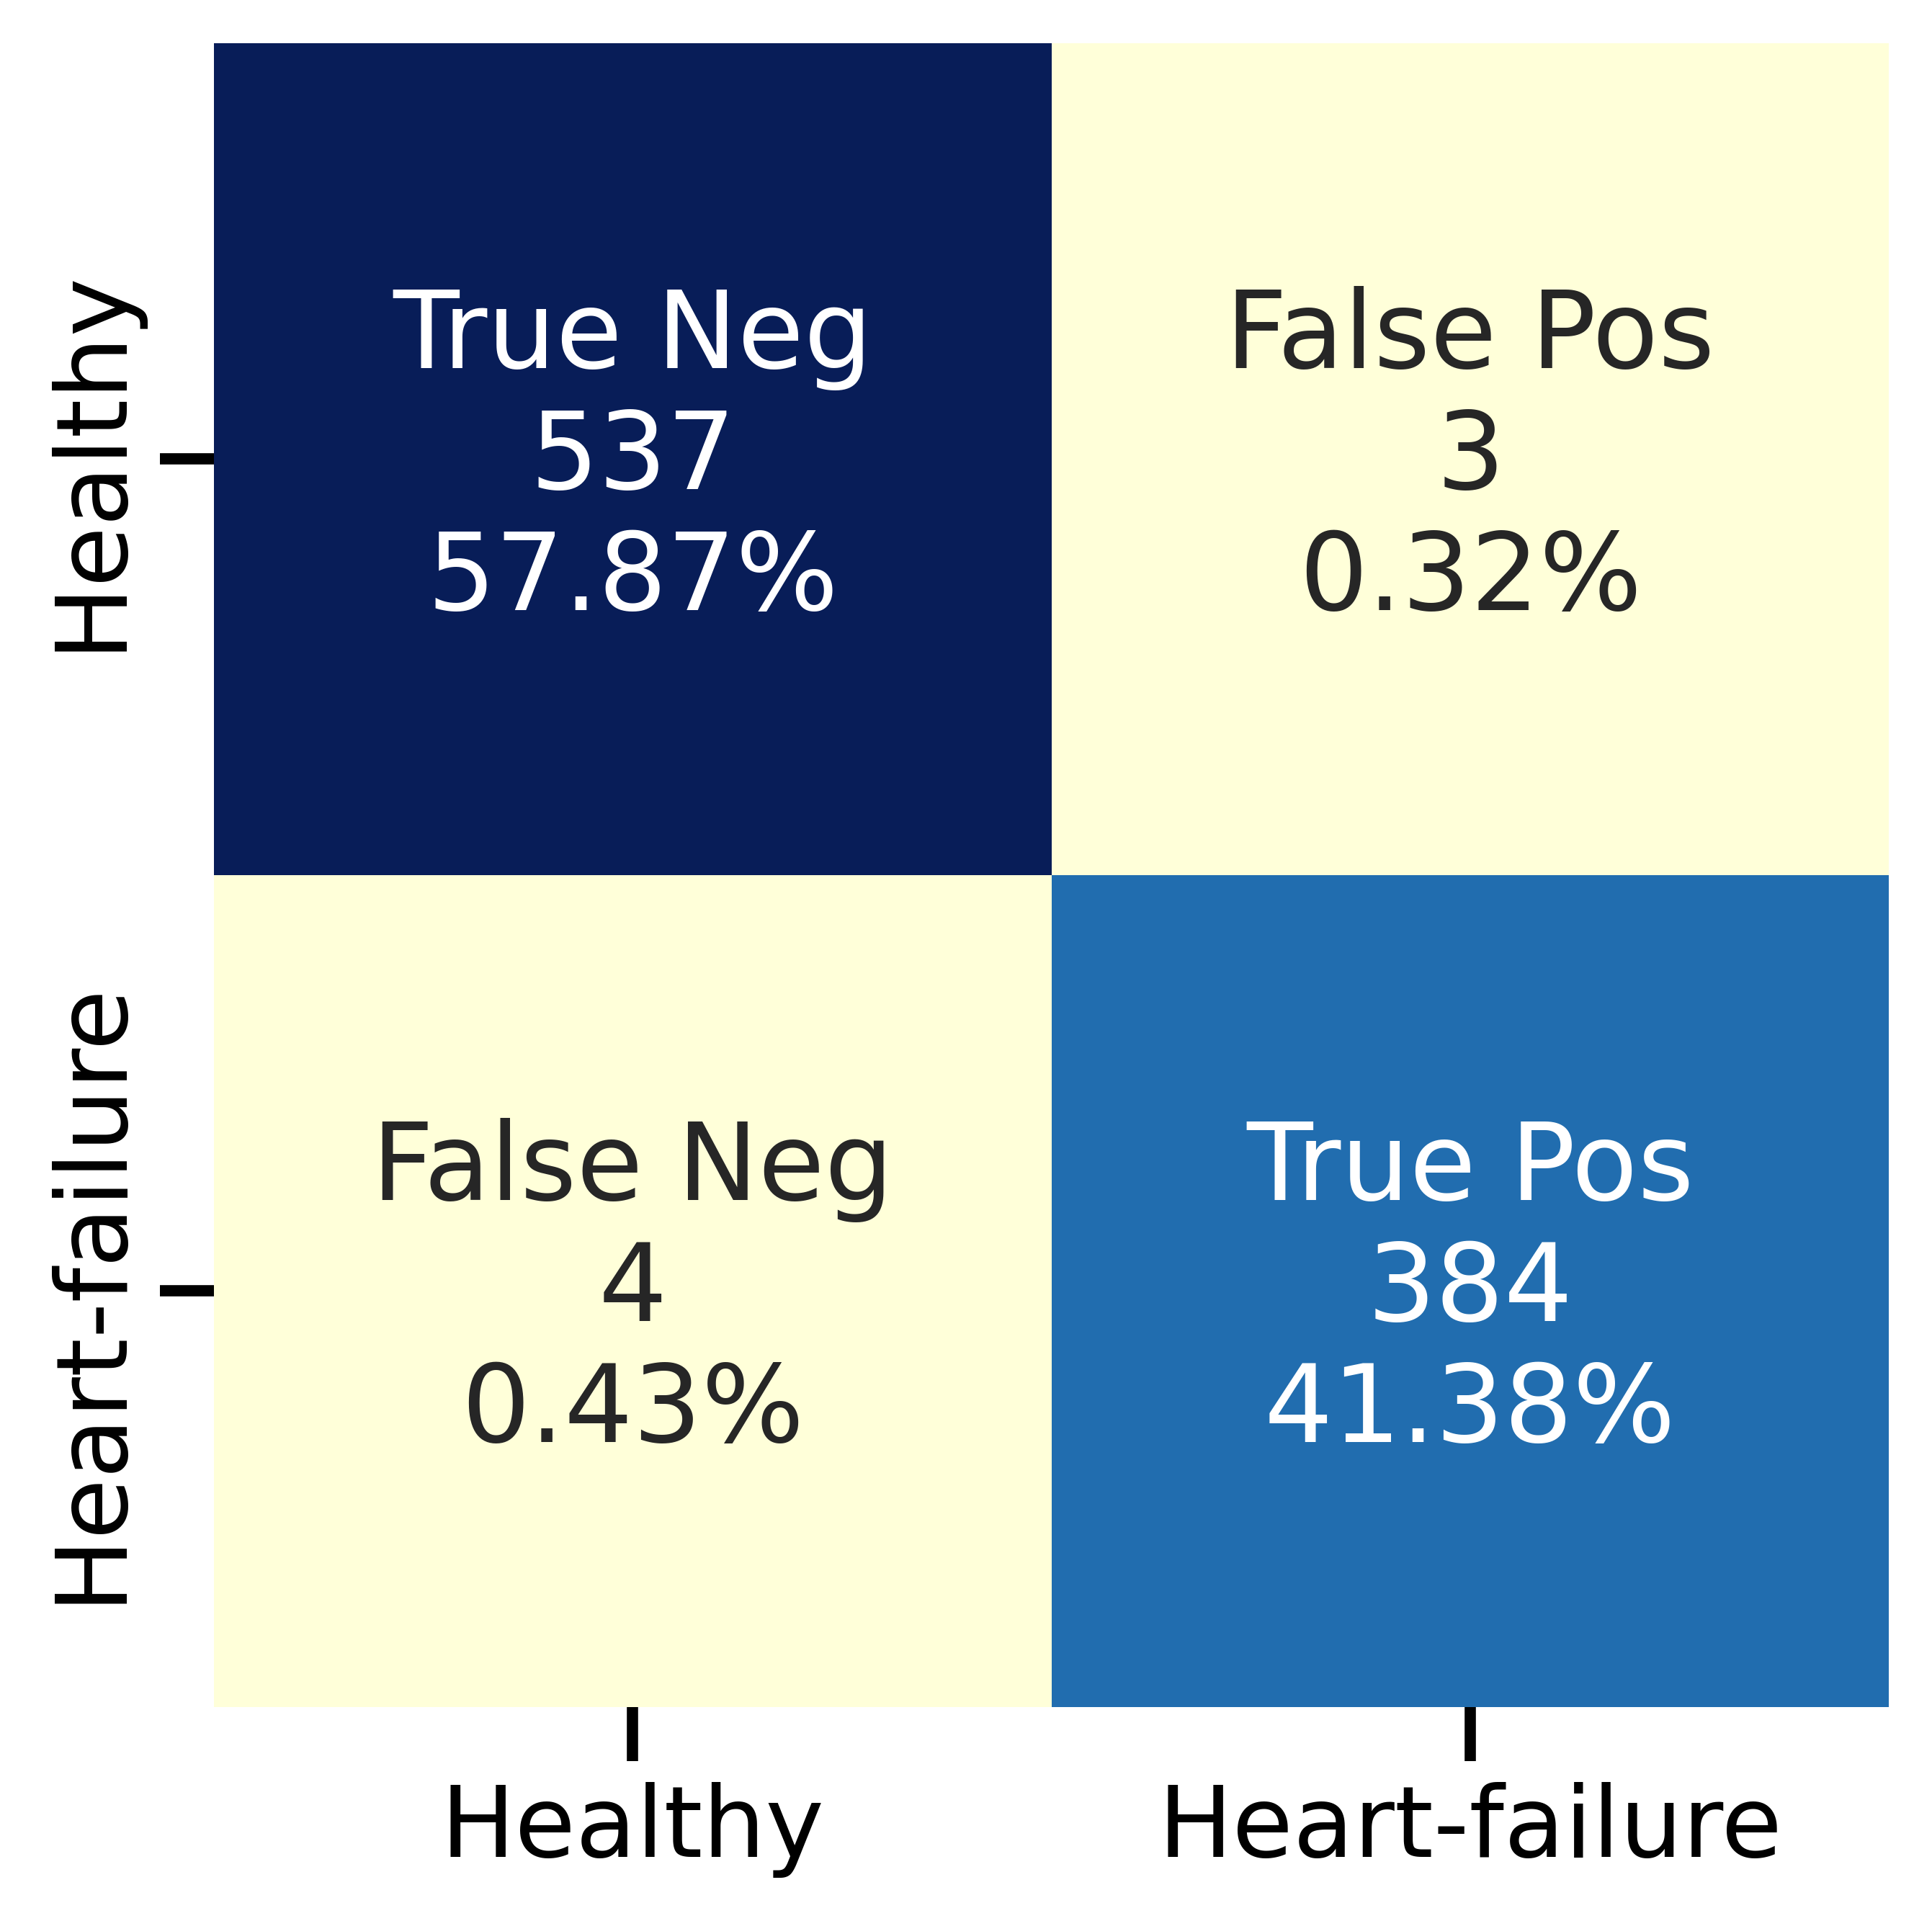
\includegraphics[width=\textwidth]{./figs/results/Confusion Matrix 2.png}
        \caption{Multi-region fusion auscultation}
        \label{fig:mitral_valve_2}
    \end{subfigure}
    \hfill
    \begin{subfigure}[b]{0.45\textwidth}
        \centering
        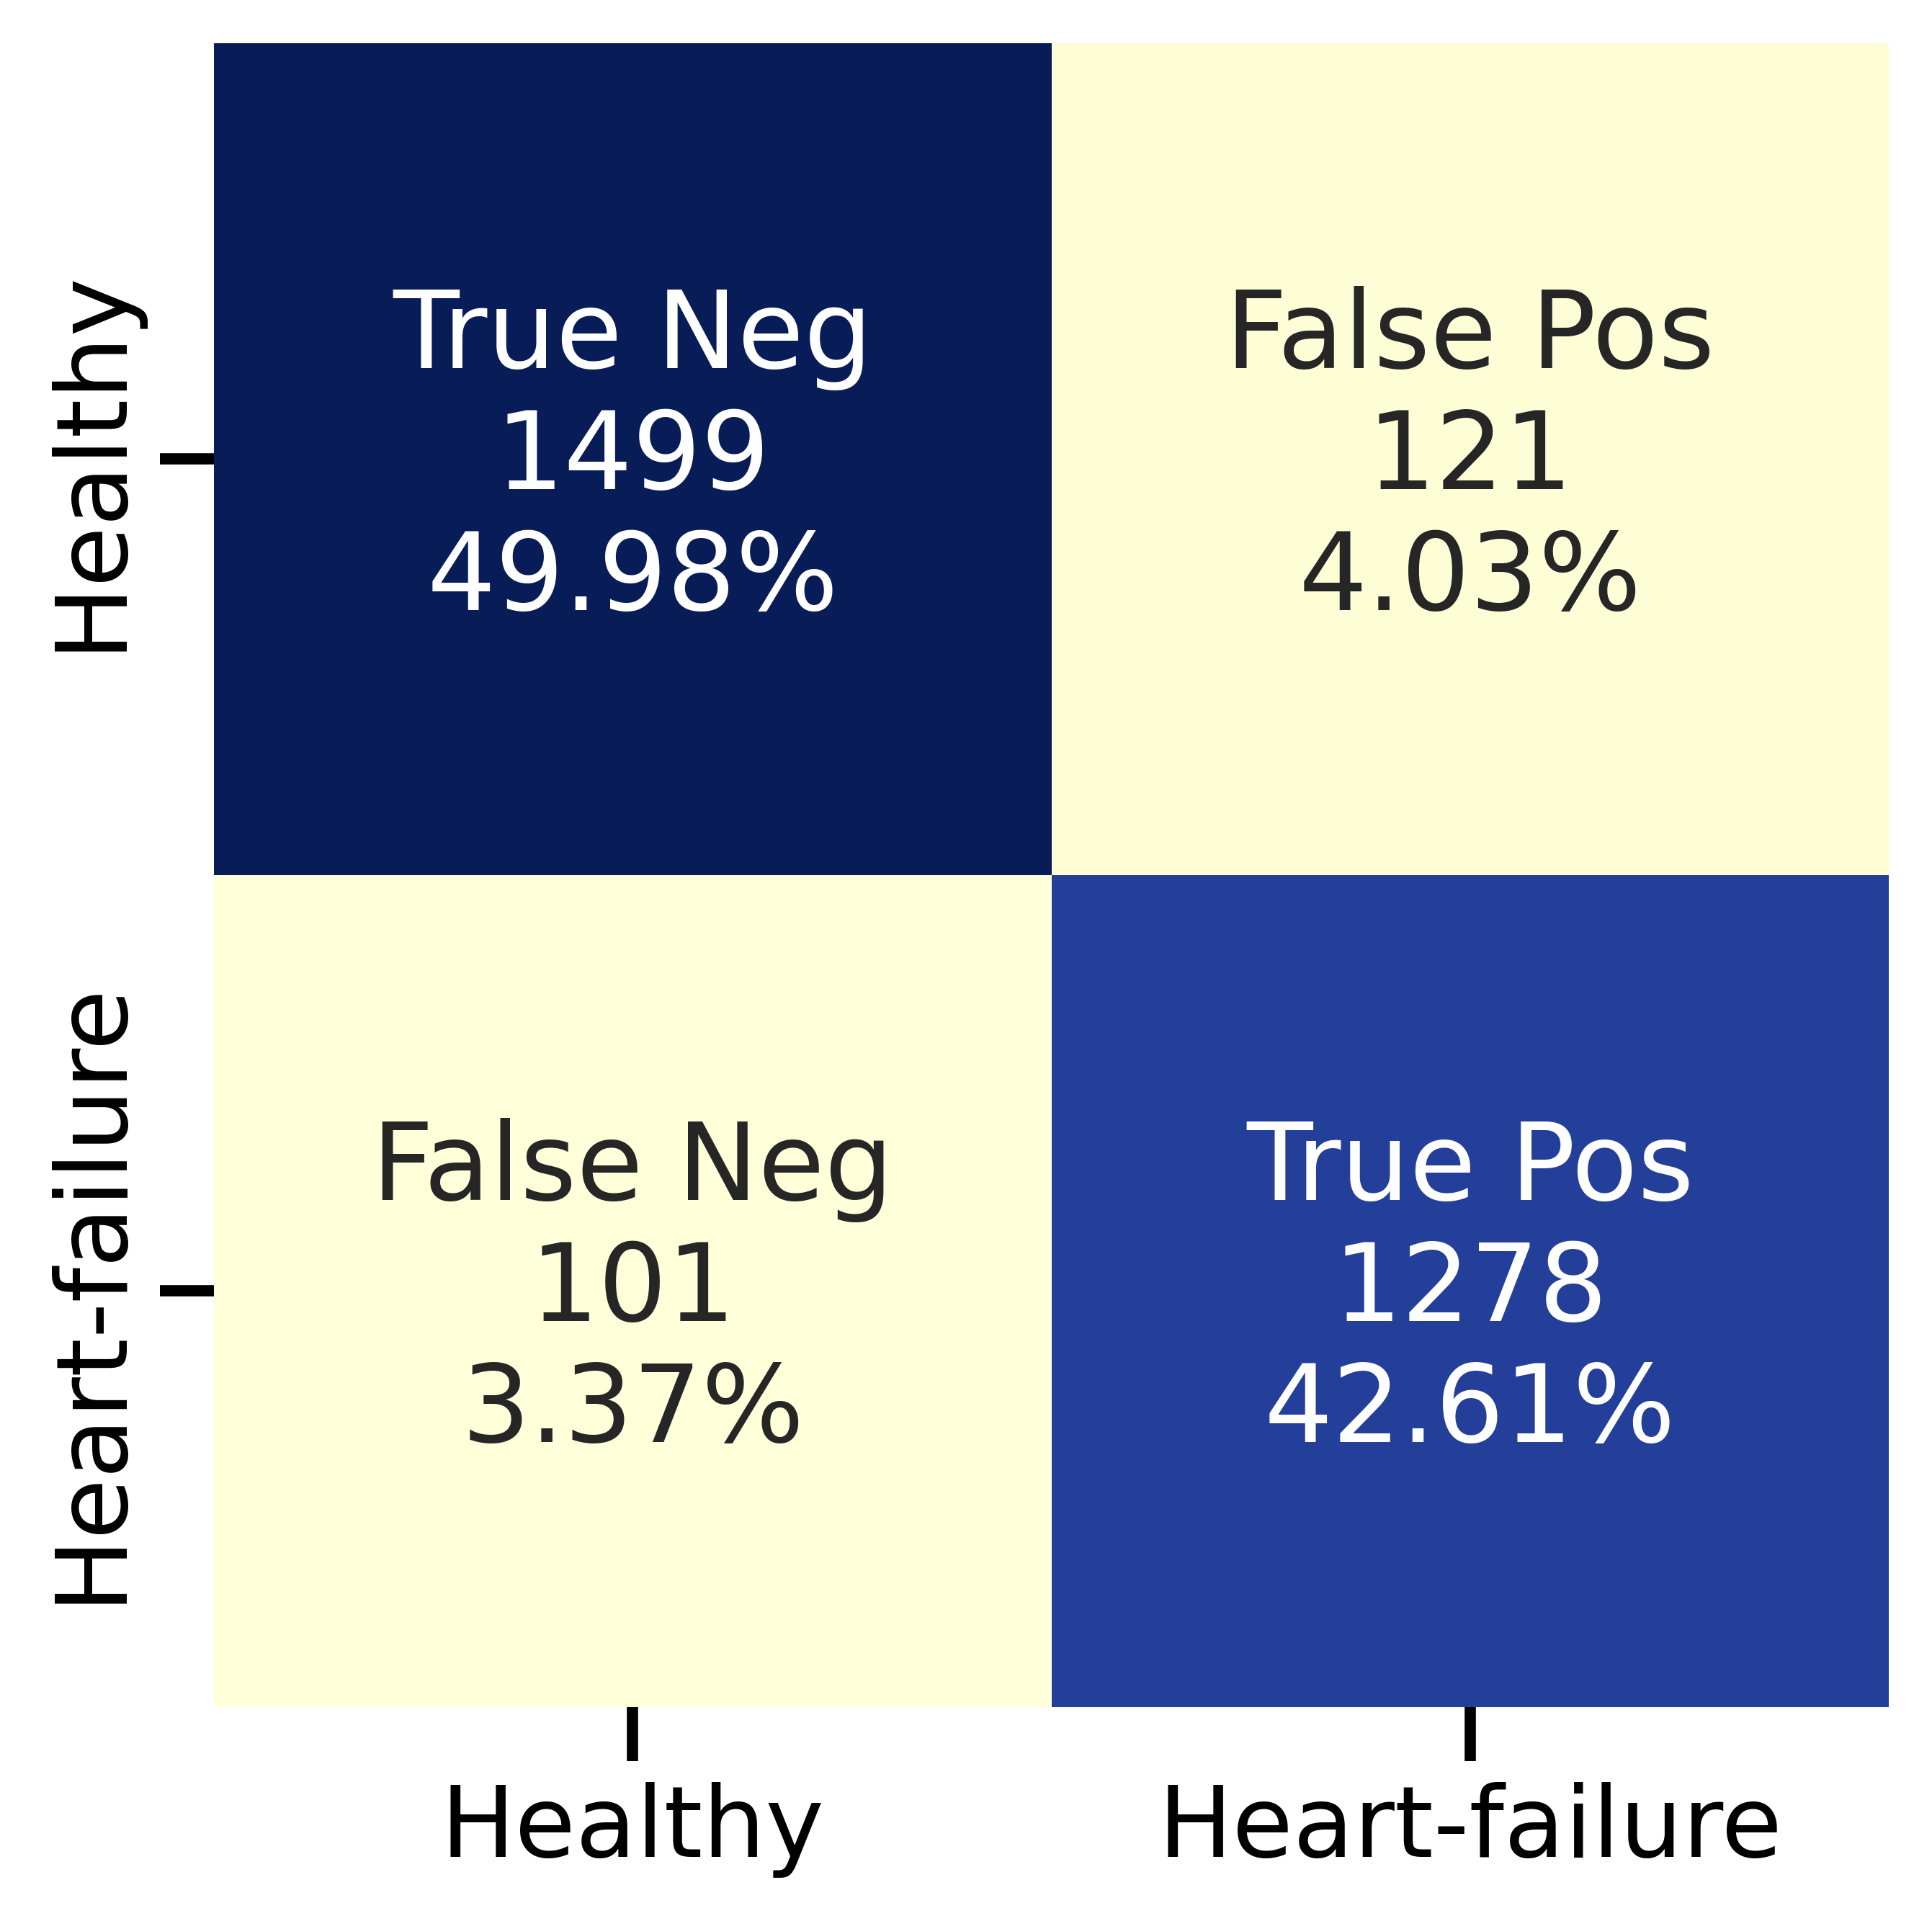
\includegraphics[width=\textwidth]{./figs/results/Confusion Matrix 1.png}
        \caption{Mitral valve auscultation}
        \label{fig:mitral_valve_1}
    \end{subfigure}
    \caption{\textbf{Comparison of two auscultation strategies}}
    \label{fig:comparison}
\end{figure*}

Tab.\ref{tab:HF Diagnosis 10-fold Results} also presents the results obtained from the Yaseen dataset. DenseHF-Net, ResNet-18, and MobileNetV1-28 typically reached convergence around 50 epochs. The AS diagnosis exhibits the best performance, with sensitivity and specificity exceeding 82\% across all three models. For MS and MR, all three models achieve correct diagnoses, with sensitivity and specificity exceeding 87\% in both ResNet-18 and MobileNetV1-28. However, MVP diagnosis by DenseHF-Net yields suboptimal results, with a specificity of only 30\% and an F1-Score of only 45.88\%.




\subsection{Mitral valve auscultation}
For mitral valve auscultation, DenseHF-Net demonstrates the best performance with an accuracy of 92.60\% ± 1.11\%, along with a good balance between sensitivity (92.68\% ± 0.88\%) and specificity (92.53\% ± 2.08\%), as shown in Tab.\ref{tab:HF Diagnosis 10-fold Results}. In comparison, ResNet-18 has slightly lower accuracy (91.33\% ± 2.48\%), with competitive sensitivity (92.32\% ± 2.59\%) but lower specificity (90.20\% ± 4.49\%), indicating a higher rate of false positives. MobileNetV1-28 shows the lowest accuracy (90.73\% ± 1.80\%) and the least balanced performance in terms of sensitivity (90.68\% ± 2.49\%) and specificity (90.80\% ± 2.97\%).

Overall, DenseHF-Net is the most effective model for mitral valve auscultation, offering superior accuracy and a better balance between sensitivity and specificity, making it the preferred choice among the three models.

Fig. \ref{fig:comparison} illustrates a comparative analysis of two different auscultation strategies, as represented by the respective confusion matrices. Both strategies focus on the detection accuracy of mitral valve abnormalities. The confusion matrices in Fig. \ref{fig:mitral_valve_1} and Fig. \ref{fig:mitral_valve_2} summarize the performance outcomes, including True Positives, True Negatives, False Positives, and False Negatives.

In the first strategy (Fig. \ref{fig:mitral_valve_1}), the model achieved a high sensitivity of 92.68\% and specificity of 92.53\%, with a balanced F1 score of 92.01\%. The second strategy (Fig. \ref{fig:mitral_valve_2}) demonstrated even higher accuracy, achieving a sensitivity of 98.97\% and a specificity of 99.44\%, leading to an F1 score of 99.10\%.

\subsection{Ablation Study}
Table 3 presents the results of the ablation study, using Params, FLOPs, MACs, and ten-fold cross-validation accuracy as evaluation metrics. 
DenseHF-Net strikes a balance between computational efficiency and performance, with 0.33 million parameters, 61.29 million FLOPs, and 30.64 million MACs, achieving an accuracy of 93.47\%.

When wavelet-denoising was not applied, the accuracy dropped to 93.26\%, indicating that wavelet-denoising has a certain positive impact on model performance. Similarly, using Mel-spectrum features resulted in a significant decrease in accuracy to 90.77\%, highlighting the crucial role of feature selection in maintaining high performance.

Adjusting the compression rate showed a clear trade-off between model complexity and accuracy. As the compression rate increased from 30\% to 70\%, the number of parameters, FLOPs, and MACs also increased, leading to a slight improvement in accuracy. However, the highest accuracy (95.1\%) was achieved without compression, which also resulted in the highest computational cost, underscoring the need to balance accuracy and efficiency.

Finally, increasing the number of blocks in the network further raised the number of parameters, FLOPs, and MACs. When the block numbers were set to 8, 16, 32, 16, the accuracy reached 94.74\%. This indicates that while deeper networks may offer higher accuracy, they also significantly increase the computational burden, which could be a limiting factor in real-time or resource-constrained applications.

In the final configuration, DenseHF-Net employed a 10\% compression rate and block numbers of 4, 8, 16, and 8. This configuration was chosen to prune the model as much as possible while maintaining performance, making it more suitable for emergency scenarios such as use in ambulances.
\begin{table*}[htbp]
    \centering
    \caption{Ablation Study Results}
    \label{table:ablation_results}
    \begin{tabularx}{\textwidth}{L|CCCCC}
    \toprule
    Ablation Condition & Params (M) & FLOPs (M) & MACs (M) & Accuracy (\%) \\ 
    \midrule
    \textbf{DenseHF-Net }           &0.33& 61.29& 30.64& 92.60 \\
    Without wavelet-denoising  &0.33& 61.29& 30.64& 92.26 \\
    Feature input: Mel-spectrum &0.33& 61.29& 30.64& 90.77\\
   Compression rate: 30\%& 0.39& 67.01& 33.50&93.87\\
   Compression rate: 50\%& 0.47& 74.13 & 37.06&93.91\\
   Compression rate: 70\%& 0.57& 82.42 & 41.21&94.01\\
   Without compression &0.78& 98.84& 49.42& 95.10\\
    Blocks numbers: 6 12 24 16  & 0.99    & 132.64     & 66.32     & 94.35  \\
    Blocks numbers: 8 16 32 16  & 1.47    & 201.76      & 100.88    & 94.74  \\
    \bottomrule
    \end{tabularx}
\end{table*}